\paragraph{} Este capítulo tem como objetivo apresentar uma breve introdução sobre o Biodiesel. Além disso, será descrito seu desenvolvimento no mercado brasileiro.

\paragraph{} O Biodiesel é um biocombustível produzido a partir de fontes renováveis como óleos vegetais e gorduras animais que reagem por meio de transesterificação com um álcool primário. Embora o biodiesel possa ser produzido a partir de várias matérias-primas, no Brasil o óleo de soja é a principal fonte de matéria-prima para a produção de biodiesel \cite{biodiesel_def_anp}, respondendo por mais de 70\% da produção.
\paragraph{} No Brasil, a introdução do biodiesel na matriz energética tem sido uma resposta tanto às questões ambientais quanto à necessidade de diversificação das fontes de energia e colocam o Brasil como referência no ramo de biocombustíveis \cite{biodiesel_esp_anp}.

\section{Vantagens em Relação ao Óleo Diesel}
\paragraph{} A substituição do Óleo Diesel pelo Biodiesel apresenta uma série de vantagens. No ponto de vista ambiental, a queima do Biodiesel B100 não libera Óxidos de Enxofre (\(SO_x\)), que são agentes causadores da chuva ácida, além de ser biodegradável, se decompondo mais rápido que combustíveis fósseis. No que diz respeito à saúde da população, sua queima gera emissões com baixa concentração de Monóxido de Carbono (\(CO\)) \cite{silva2023biodiesel}, que pode causar sérios problemas respiratórios e cardiovasculares. Além disso, pode ser usado em motores a diesel convencionais sem a necessidade de grandes modificações \cite{totalenergies_biodiesel}.
\paragraph{} O biodiesel apresenta uma vantagem significativa em relação à pegada de carbono devido ao seu ciclo de \(CO_2\) relativamente curto. O dióxido de carbono emitido durante a queima do biodiesel é compensado pela fotossíntese das plantas que fornecem as matérias-primas \cite{silva2023biodiesel}, o que contribui para a minimização dos impactos no aquecimento global.
\paragraph{} Em contrapartida, sua produção depende do uso de terras agrícolas \cite{totalenergies_biodiesel} e de produtos da cesta básica, como o óleo de soja \cite{infomoney_cesta_basica}, provocando aumento nos preços. O biodiesel também é mais corrosivo e sujeito a degradação do que os combustíveis fósseis, o que pode provocar problemas em motores mais antigos que ainda possuem componentes feitos de materiais como plásticos, metais e borrachas de origem natural \cite{totalenergies_biodiesel}.

\section{Produção de Biodiesel no Brasil}

\paragraph{}A produção de biodiesel no Brasil começou a ganhar impulso no início dos anos 2000, com a implementação do \ac{PNPB}.

\paragraph{}Segundo a \ac{ANP}, a produção de biodiesel no Brasil alcançou cerca de 7,5 bilhões de litros em 2023 \cite{ANPBoletim12_2023}, em 2024 espera-se produzir 10 bilhões de litros \cite{ANPBoletim01_2024}.

\section{Regulação e Início do Mercado}

\paragraph{} O \ac{PNPB}, criado em 2004, foi o marco inicial para a regulamentação do biodiesel no Brasil. Este programa foi essencial para estabelecer as bases legais e econômicas para a produção e comercialização do biodiesel. Em 2005, foi autorizada a mistura de biodiesel ao diesel, até 2\%. Em 2008, a mistura se tornou obrigatória, em 2\% (B2), aumentando gradualmente ao longo dos anos \cite{biodiesel_def_anp}.
\paragraph{} Inicialmente, as vendas eram exclusivamente por meio de leilões realizados pela \ac{ANP}. A partir de 2021, foi autorizada a compra diretamente com os fornecedores com venda bimestral regulada pela \ac{ANP} \cite{epbr2021}.

\begin{figure}
	\begin{center}
		\parbox[htb]{13.0cm}
		{
			\begin{center}
				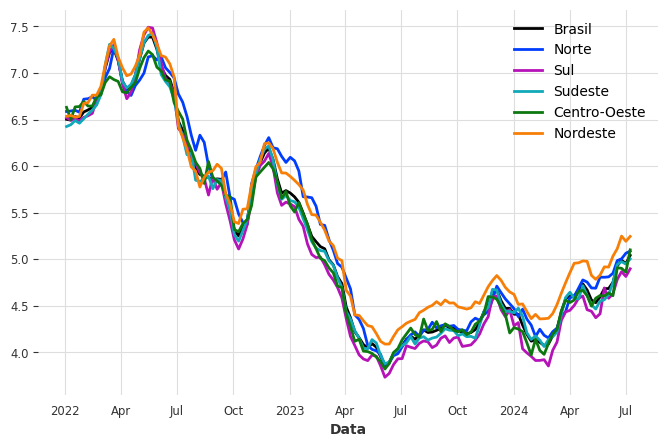
\includegraphics[width=0.8\textwidth]{figuras/biodiesel_price.png}
				\caption{Série de Preços do Biodiesel no Brasil (R\$/litro) a partir de 2022}
				\label{fig:biodiesel_price}
				\text{Fonte: Elaborado pelo autor, baseado em \ac{ANP} \cite{biodiesel24}}
			\end{center}
		}
	\end{center}
\end{figure}

\subsection{Percentuais de Adição no Diesel}

\paragraph{} A mistura obrigatória de biodiesel no diesel tem sido aumentada progressivamente desde sua criação, se adaptando a oferta das matérias primas e ao desenvolvimento das tecnologias de produção.
\paragraph{} Devido à crise de oferta de soja em 2020 aliada ao aumento do \ac{IPCA}, o percentual de mistura foi reduzido de 12\% para 10\% em setembro de 2020 para reduzir os efeitos da crise. Em 2023, o percentual de mistura de biodiesel no diesel volta a subir \cite{g12020} de acordo com o planejamento da \ac{ANP}. Além disso, a recente Lei 14.993, de 2024 \cite{lei14993}, sancionada pelo presidente da república, estabelece novos percentuais crescentes para a mistura de biodiesel no diesel, como parte da estratégia nacional para promover os chamados "combustíveis do futuro" \cite{senadonoticias}. 
\paragraph{} Atualmente, especialistas acreditam que a produção é capaz de atender a demanda de uma mistura de 20\% de biodiesel no óleo diesel e com potencial para chegar a 25\% \cite{canalrural_biodiesel}, ainda longe das projeções da \ac{ANP}, como mostrado na Tabela \ref{tab:mistura_biodiesel}.


\begin{table}[htbp]
	\begin{center}
		\caption{Percentual de Mistura de Biodiesel no Brasil ao Longo do Tempo}
		\label{tab:mistura_biodiesel}
		\begin{tabular}{|c|c|}
	\hline
	\textbf{Período}                       & \textbf{Percentual de Mistura (\%)} \\
	\hline
	01/2005 - 12/2007\textsuperscript{*}   & 2                                   \\
	01/2008 - 06/2008                      & 2                                   \\
	07/2008 - 06/2009                      & 3                                   \\
	07/2009 - 12/2009                      & 4                                   \\
	01/2010 - 06/2014                      & 5                                   \\
	07/2014 - 10/2014                      & 6                                   \\
	11/2014 - 02/2017                      & 7                                   \\
	03/2017 - 02/2018                      & 8                                   \\
	03/2018 - 08/2019                      & 10                                  \\
	09/2019 - 02/2020                      & 11                                  \\
	03/2020 - 08/2020                      & 12                                  \\
	09/2020 - 10/2020\textsuperscript{**}  & 10                                  \\
	11/2020 - 12/2020                      & 11                                  \\
	01/2021 - 02/2021                      & 12                                  \\
	03/2021 - 04/2021                      & 13                                  \\
	05/2021 - 08/2021\textsuperscript{**}  & 10                                  \\
	09/2021 - 10/2021                      & 12                                  \\
	11/2021 - 03/2023\textsuperscript{**}  & 10                                  \\
	04/2023 - 03/2024                      & 12                                  \\
	04/2024 - 02/2025\textsuperscript{***} & 13                                  \\
	03/2025 - 02/2026\textsuperscript{***} & 15                                  \\
	03/2026 - 02/2027\textsuperscript{***} & 16                                  \\
	03/2027 - 02/2028\textsuperscript{***} & 17                                  \\
	03/2028 - 02/2029\textsuperscript{***} & 18                                  \\
	03/2029 - 02/2030\textsuperscript{***} & 19                                  \\
	03/2030\textsuperscript{***} 		   & 20                                 \\
	\hline
\end{tabular}
		\begin{minipage}{\textwidth}
			\footnotesize
			\textsuperscript{*} Percentual de mistura de biodiesel facultativo. \\
			\textsuperscript{**} Queda no percentual obrigatório devido à escassez de soja \cite{g12020}. \\
			\textsuperscript{***} Projeção. \\
		\end{minipage}
		\text{Fonte: \ac{ANP} \cite{biodiesel_esp_anp} e Lei 14.993, de 2024 \cite{lei14993}}
	\end{center}
\end{table}

\subsubsection{Biodiesel 100\% (B100)}

A \ac{ANP} regula o uso experimental do biodiesel B100 através de resoluções específicas. Para utilizar B100 experimentalmente, é necessário obter a prévia anuência da ANP, apresentando um projeto detalhado que especifica o objetivo do experimento, os volumes a serem utilizados, a logística envolvida, os riscos e as medidas de mitigação \cite{ANP910_2022}.